\chapter{Detecção de fraude}

Existem dois tipos principais de fraude, de acordo com o autor: interna e externa. Em um documento de 2012 \cite{ACFE2012}, a Associação de Investigadores de Fraude Certificados (Association of Certified Fraud Examiners, ACFE) definiu a fraude interna como ``a exploração ilegal dos recursos e bens de uma empresa, por um empregado, para enriquecimento próprio''\footnote{The use of one’s occupation for personal enrichment through the deliberate misuse or misapplication of the employing organization’s resources or assets.}.

Os autores da fraude externa dividem-se em três perfis: casual, criminal e crime organizado \cite{Phua2010}. Criminosos casuais apresentam comportamento aleatório, transgredindo as leis quando têm oportunidade, tentação ou em períodos de dificuldades financeiras. Por outro lado, indivíduos ou grupos organizados são mais perigosos porque tentam esconder ou dissimular sua verdadeira identidade, além de evoluir seu \emph{modus operandi} com o tempo, tentando burlar os sistemas de detecção e evitar a sua identificação. Assim, é importante levar-se em consideração essa constante interação entre os sistemas de detecção e os fraudadores profissionais.

O monitoramento de sistemas com o objetivo de encontrar comportamentos fraudulentos já existia muito antes da utilização de sistemas computacionais tornarem-se ferramentas comuns. Antes havia um processo denominado auditoria: gerar, armazenar e revisar um registro cronológico de eventos de um sistema \cite[p. 7]{Bace2000}. Os principais objetivos desses sistemas são identificar os usuários do sistema, impedir o uso impróprio, e auxiliar na reconstrução de eventos e na estimativa, quantificação e qualificação de danos.

O primeiro trabalho a considerar necessária a auditoria automática de sistemas foi \citet{Anderson1972}. Nesse trabalho, Anderson classifica os riscos e ameaças a sistemas, diferenciando fontes internas e externas, como na figura \ref{fig:and}. Também cita diversos objetivos para um sistema de auditoria:

\begin{itemize}
\item Prover informações suficientes para que o problema possa ser localizado, mas que não exponham detalhes que possibilitem um ataque.
\item Obter dados de diversas fontes para otimizar o conteúdo do banco de dados.
\item Discernir uma atuvidade ``normal'' do sistema, para que se possa detectar abusos interno.
\item Levar em consideração as estratégias dos invasores no projeto do sistema.
\end{itemize}

\begin{figure}[h]
\centering
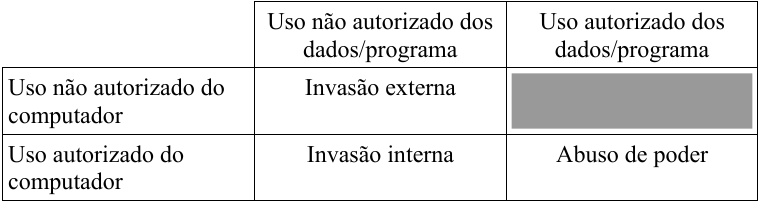
\includegraphics[width=0.75\textwidth]{img/anderson.png}
\caption{Matriz de ameaças}
\label{fig:and}
\end{figure}

\ldots

A detecção de fraude é apenas uma das etapas de um sistema chamado de \emph{controle de fraude}. Nesse contexto, a detecção automática ajuda a reduzir o trabalho manual de verificação das instâncias. O objetivo principal desses sistemas é identificar padrões de transações suspeitas em meio às transações comuns de uma organização. O fraudador pode, por exemplo, contratar um seguro usando informações de outra pessoa ou informações falsas.

Como não é possível ter certeza da legitimidade das transações de um negócio, não existe uma técnica infalível para a detecção de fraudes. Isso não significa que elas não possam ser detectadas. Métodos matemáticos e estatísticos são utilizados para comparar um banco de dados de transações existentes com as novas, com o objetivo de encontrar evidências de possíveis fraudes. Mesmo assim, geralmente há um processo de análise e revisão caso a caso por um especialista.

Dois conceitos relacionados à detecção em geral são falsos positivos e falsos negativos. Falsos positivos são instâncias erroneamente classificadas, por exemplo, uma transação comum que é classificada como fraudulenta. Falsos positivos são o oposto: uma transação fraudulenta que é classificada como comum. O número de falsos positivos aumenta o trabalho desnecessário na fase de revisão, enquanto os falsos negativos reduzem a eficácia da detecção. A redução dos falsos positivos é um dos objetivos principais de um sistema de detecção. Os falsos negativos, no entanto, são quase impossíveis de serem eliminados completamente, em qualquer sistema de detecção.

Mesmo um sistema capaz de reconhecer sinais de fraudes existentes não é suficiente para um ambiente real. Fraudadores tentam constantemente superar os sistemas de detecção, evoluindo o se \emph{modus operandi} com o tempo, novos métodos são criados, novos fraudadores entram em atividade. Um sistema que almeje deter o maior número possível deve ser constantemente atualizado para se adaptar às mudanças de um ambiente tão dinâmico.

Dependendo do domínio da organização, para que um sistema possa prever fraudes com antecedência suficiente para que elas sejam evitadas, deve monitorar constantemente as novas transações em andamento. Esse fator reduz a utilização de sistemas que necessitam de um longo tempo de treinamento ou de análise. O ideal seria que ele estivesse em constante execução, analisando as transações conforme elas ocorrem. Para aplicações grandes ou descentralizadas, pode ser muito difícil conseguir isso sem afetar a performance geral das transações.

Para cada domínio, tipos diferentes de fraude podem existir, e mais de um tipo pode ocorrer simultaneamente, sem uma ordem definida. 

\section{Dados}

Os atributos das instâncias em um banco de dados usado para detecção de fraude geralmente limitam-se a valores binários, numéricos, categóricos ou uma mistura desses três. Os atributos usados são semelhantes. Aplicações de seguro utilizam o histórico do cliente: tempo de contrato, histórico e total de pagamentos, lucro anual valor médio depositado em conta bancária. Para fraudes de crédito, informações sobre as transações: valor, data, localização geográfica, conta de destino, tempo de conta.

O número de instâncias positivas nesse tipo de bases de dados é geralmente muito reduzido: as fraudes representam um percentual muito pequeno em relação ao número de transações legítimas de uma organização, geralmente menor do que 20\%. Métodos de detecção de fraude nunca são perfeitos: deve existir um mecanismo para lidar com as fraudes que não são identificadas a tempo de serem impedidas.

A obtenção de bancos de dados reais para teste é difícil, já que empresas e organizações, por razões legais e competitvas não disponibilizam informações desse tipo. Uma alternativa é a criação de um banco de dados artificial, inspirado em dados reais. A eficácia dessa técnica é limitada pela capacidade do criador do banco em prever o maior número de casos possíveis, o que geralmente é muito inferior à variedade das situações reais. Mesmo assim, essa técnica é comumente empregada na fase de concepção e teste, devido à dificuldade de obtenção de dados.

